\section{Results}
\label{sec:Results}

\subsection{Parmater Search}

The parameter search for the optimal C and $\sigma$ parameters is shown in the contour plots of Figures \ref{fig:ParamLiver}, \ref{fig:ParamGlass} and \ref{fig:ParamGlass}.
The optimal classifier parameters are shown in Table \ref{tab:ParamValues}.
\todo{Make some quantifications and discuss the data}
\begin{table}[ht!]
\caption{Optimal Classifier Parameters}
\label{tab:ParamValues}
\begin{tabular}{c c c c c c c c}
\hline
Data Set & $C_{min}$ & $C_{max}$ & $\sigma_{min}$ & $\sigma_{max}$ & $C$ & $\sigma$ & $\epsilon$ \\
\hline

\hline
\end{tabular}
\end{table}
\begin{figure*}[ht!]
	\centering
	\begin{subfigure}[b]{0.45\textwidth}
		\centering
		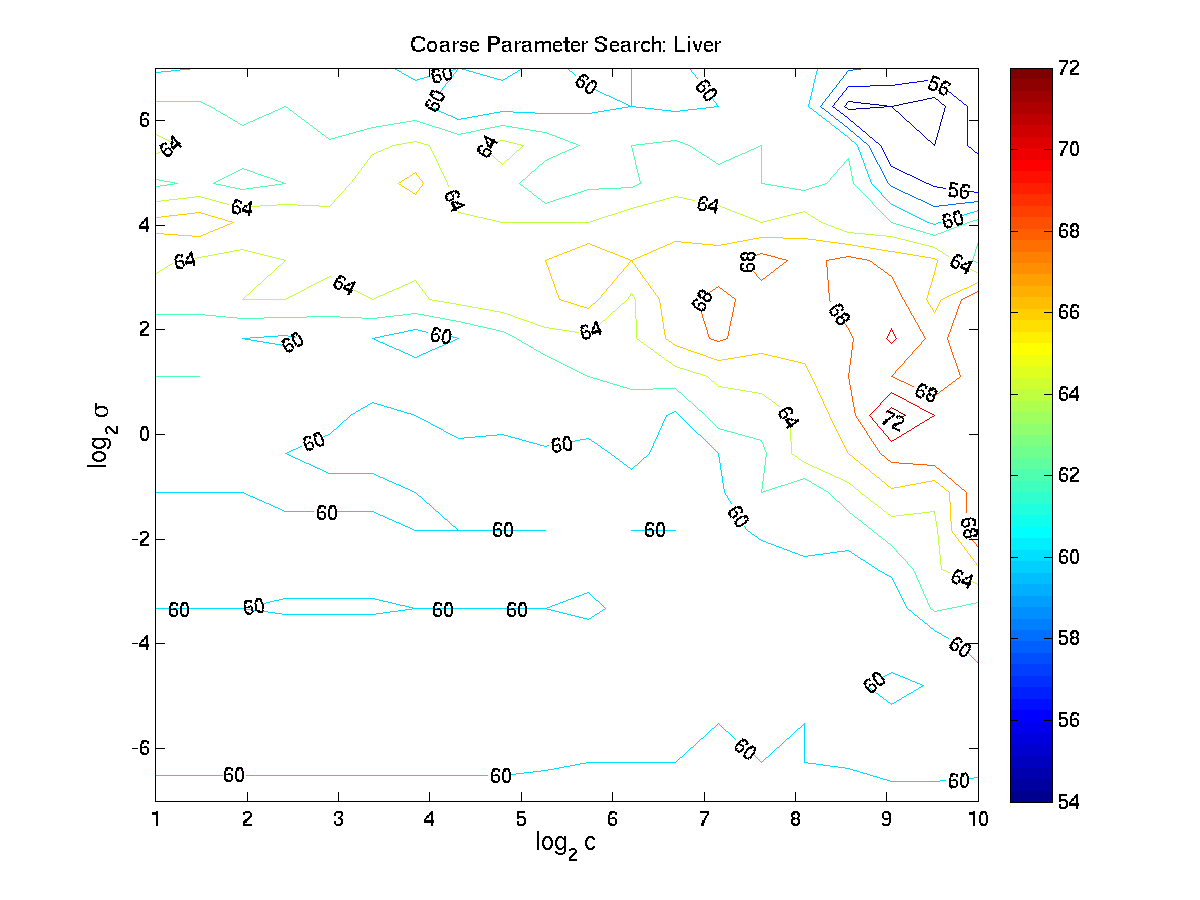
\includegraphics[width=\textwidth]{Liver_coarseSearch}
        \caption{Coarse Search}
	\end{subfigure}%
	~
	\begin{subfigure}[b]{0.45\textwidth}
		\centering
		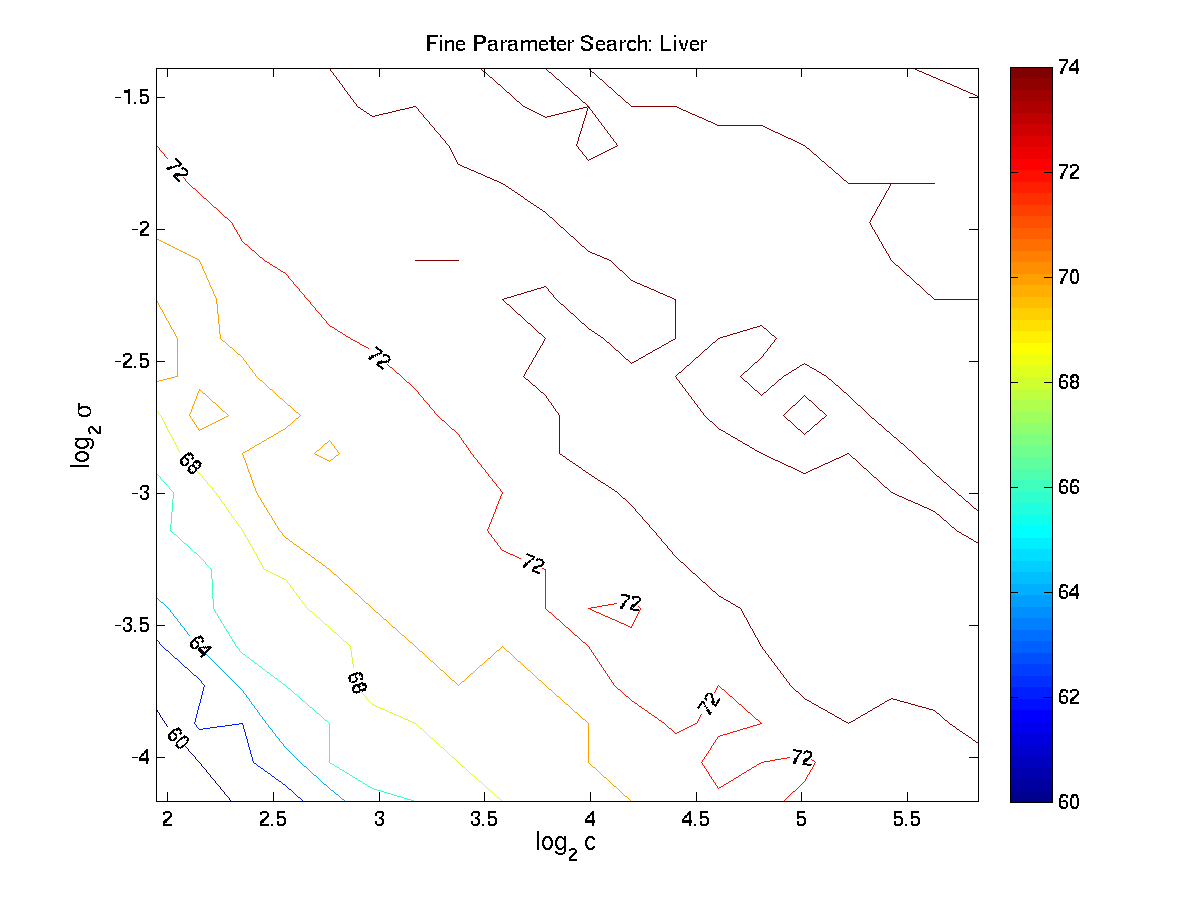
\includegraphics[width=\textwidth]{Liver_fineSearch}
        \caption{Fine Search}
	\end{subfigure}	
	\caption{Parameter search for Liver Disorder}
	\label{fig:ParamLiver}

	\begin{subfigure}[b]{0.45\textwidth}
		\centering
		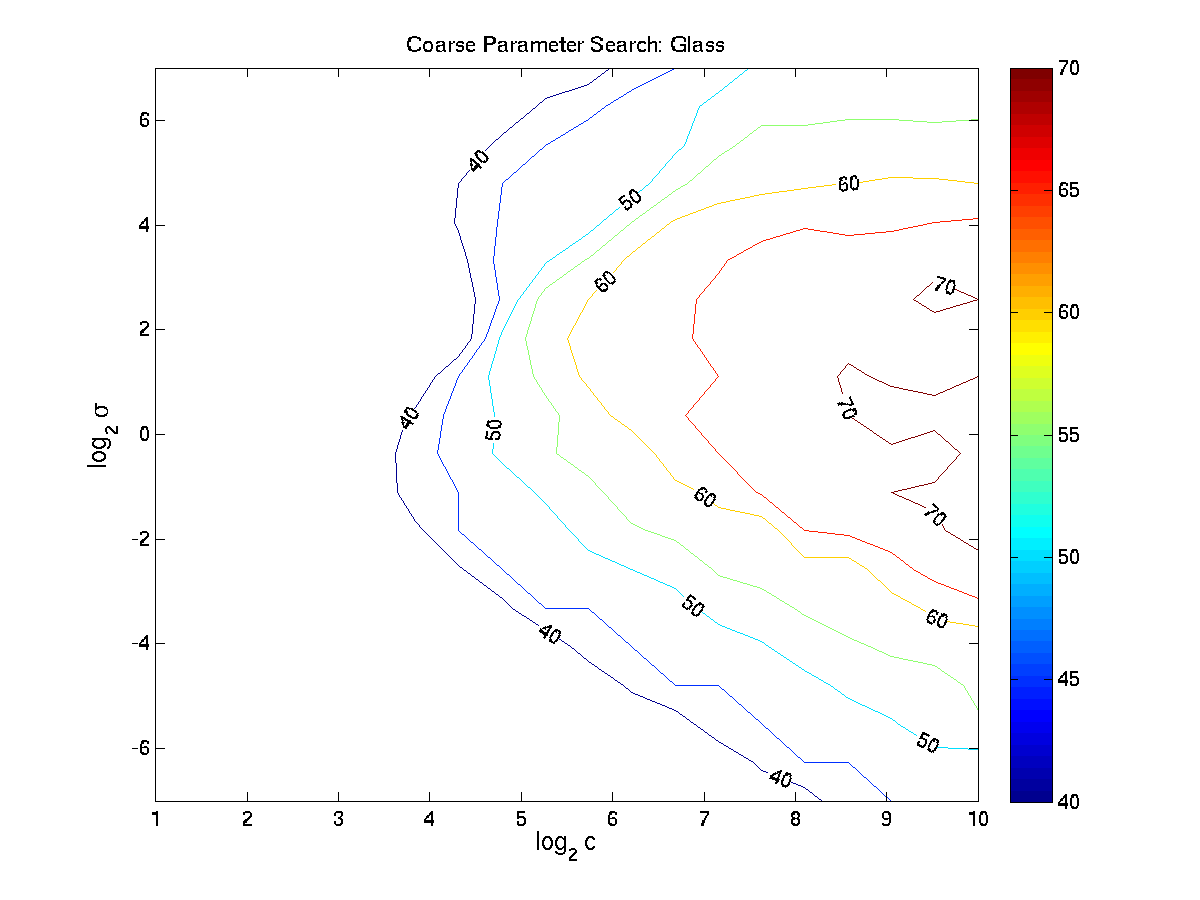
\includegraphics[width=\textwidth]{Glass_coarseSearch}
        \caption{Coarse Search}
	\end{subfigure}%
	~
	\begin{subfigure}[b]{0.45\textwidth}
		\centering
		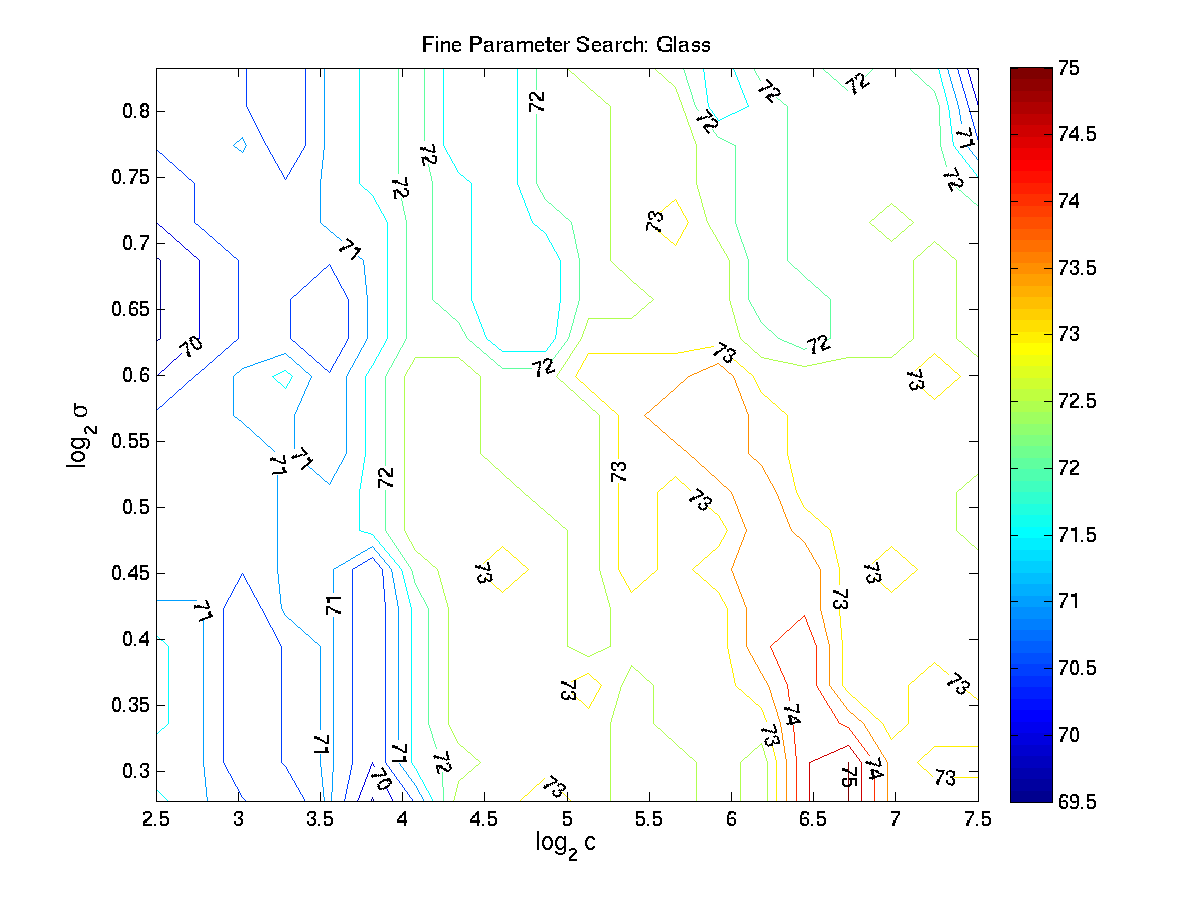
\includegraphics[width=\textwidth]{Glass_fineSearch}
        \caption{Fine Search}
	\end{subfigure}	
	\caption{Parameter search for Glass Disorder}
	\label{fig:ParamGlass}

	\begin{subfigure}[b]{0.45\textwidth}
		\centering
		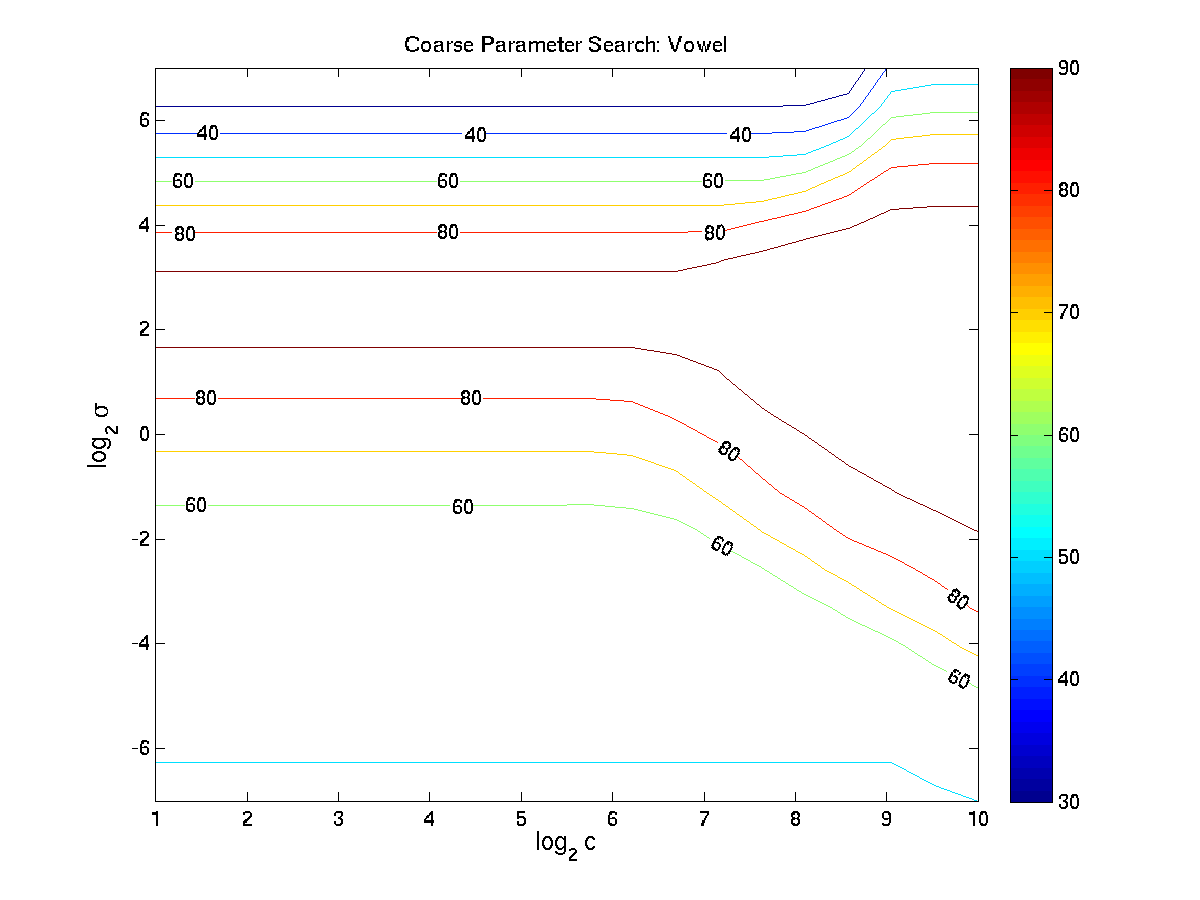
\includegraphics[width=\textwidth]{Vowel_coarseSearch}
        \caption{Coarse Search}
	\end{subfigure}%
	~
	\begin{subfigure}[b]{0.45\textwidth}
		\centering
		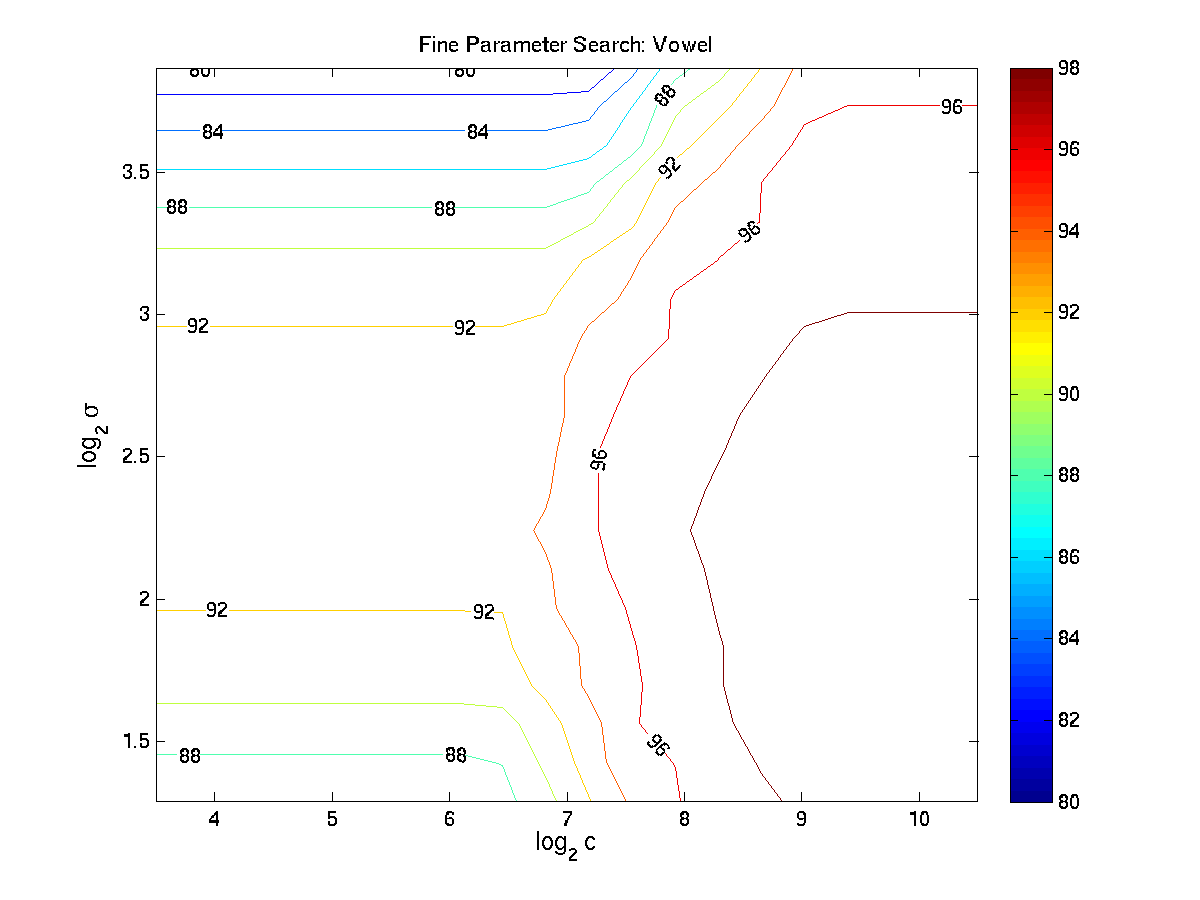
\includegraphics[width=\textwidth]{Vowel_fineSearch}
        \caption{Fine Search}
	\end{subfigure}	
	\caption{Parameter search for Vowel Disorder}
	\label{fig:ParamVowel}
\end{figure*}

\subsection{AdaBoostM1}
